\documentclass[t]{beamer}

\usepackage[slovene]{babel}
\usepackage[T1]{fontenc}
\usepackage[utf8]{inputenc}
\usepackage{amssymb}
\usepackage{amsmath}


\usepackage{lmodern}                           
\renewcommand\textbullet{\ensuremath{\bullet}}
\title{Krožnica v racionalni Bezierjevi obliki}
\author{Anja Kišek, Samo Kralj}

\usetheme{CambridgeUS}

\begin{document}
%%%%%%%%%%%%%%%%%%%%%%%%%%%%%%%%%%%%%%
\begin{frame}
\titlepage
\end{frame}

%%%%%%%%%%%%%%%%%%%%%%%%%%%%%%%%%%%%%

\begin{frame}
Vsebina:
\begin{itemize}
\item Definicija racionalnih Bezierjevih krivulj

\item Konstrukcija sklenjene krožnice s krivuljami stopnje 2,3,4

\item Krožni loki v racionalni Bezierjevi obliki

\item Kubični polkrogi

\end{itemize}

\end{frame}
%%%%%%%%%%%%%%%%%%%%%%%%%%%%%%%%%%%%
\begin{frame}
Racionalna Bezierjeva krivulja $C(t)$ stopnje $n$ v $\mathbb{R}^d$ je projekcija polinomske Bezierjeve krivulje $\tilde{C}(t)$stopnje $n$ v $\mathbb{R}^{d+1}$ na hiperravnino $w=1$, kjer je točka v $\mathbb{R}^{d+1}$ označena z $
\begin{bmatrix} x \\ w \end{bmatrix}.$


Racionalna B. krivulja stopnje $n$ je tako podana s predpisom
$$r(t) = \frac{\sum_{i=0}^n w_ib_iB_i^n(t)}{\sum_{i=0}^n w_iB_i^n(t)} $$

\end{frame}
%%%%%%%%%%%%%%%%%%%%%%%%%%%%%
\begin{frame}
Racionalna krivulja $C(t) = (X(t), Y(t))$ lahko eksaktno opiše krožnico kot projekcijo krivulje
$\tilde{C}(t) = (\tilde{X}(t), \tilde{Y}(t), W(t)),$ ki leži na stožcu, na ravnino $w = 1$.

\begin{align*}
X(t)^2 + Y(t)^2 &= 1 \\
\Big{(}\frac{\tilde{X}(t)}{W(t)}\Big{)}^2 + \Big{(}\frac{\tilde{Y}(t)}{W(t)}\Big{)}^2 &= 1\\
\tilde{X}(t)^2 + \tilde{Y}(t)^2 - W(t)^2 &= 0
\end{align*}
\begin{figure}
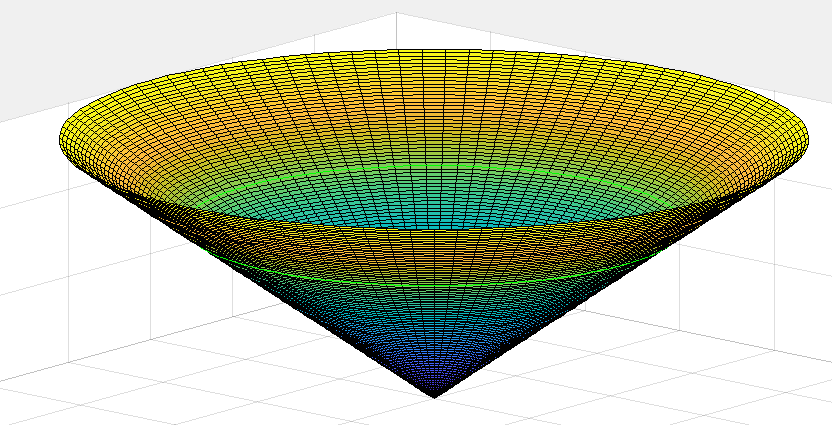
\includegraphics[scale=0.2]{stozec.png}
\end{figure}

\end{frame}

%%%%%%%%%%%%%%%%%%%%%%%%%%%%%

\begin{frame}
\textbf{Bezierjeva krivulja kot sklenjena krožnica}

Ali lahko krožnico zapišemo kot racionalno Bezierjevo krivuljo določene stopnje?
\begin{itemize}
\item Kvadratična krivulja: Ne

Zlepek krožnih lokov s kontrolnimi točkami:
\begin{align*}
\tilde{P}_0 &= (cos(\phi), -sin(\phi), 1)\\
\tilde{P}_1 &= (1, 0, cos(\phi))\\
\tilde{P}_2 &= (cos(\phi), sin(\phi), 1)
\end{align*}

\item Kubična krivulja: Ne
\end{itemize}
\end{frame}
%%%%%%%%%%%%%%%%%%%%%%%%%%%%%%%%%%%%%%



\end{document}
